%% Section 4: Constraint-Aware Replay Model
%% STATUS: STUB — not yet drafted.
%% See artifacts/revision2/SIGMETRICS_OUTLINE.md §4 for planned content (~2.5 pages).

\section{Constraint-Aware Replay Model}
\label{sec:model}

\subsection{Model Overview}
% Stateful replay of 2,637-job base workload.
% source: artifacts/phase1/analysis/phase3b_mc_results.json
% Cabinet-level thermal budget reconstruction from raw telemetry.
% Capacity yield crossing: lambda at which thermal budget becomes binding.

\subsection{Cabinet Power Model}
% Uniform per-cabinet power approximation from job-level mean power.
% Validation: 60 sampled jobs (20 small + 20 medium + 20 large).
% source: artifacts/revision1/results/power_validation_60job.json
%   overall.mae_kW = 0.3722548980702776 -> 0.37 kW
%   P99 spread = 48.21 kW -> 0.77% ~ 0.8% of spread

\subsection{Scheduling Policies}
% Policies evaluated: full_fp, full_random, fp_spread, random_spread,
%                     fp_global_placebo, fp_withincab_placebo, position_template.
% Beta parameter: BETA_F_FROZEN = 1.12484352 (original).
% Review-2 primary: PRIMARY_BETA_CHALLENGE = 1.11416358 (LOO CF median).
% source: artifacts/revision2/loo_beta_results.json (B3_primary_beta)

\subsection{Capacity Metric}
% delta_lo = C_lower(A) - C_upper(B): conservative bracket separation.
% Positive delta_lo: A's lower capacity bound exceeds B's upper bound.
% 5,000 bootstrap replicates, seed 9999, percentile CI.
% source: artifacts/revision2/challenge_analysis.json (bootstrap_seed=9999, n_bootstrap=5000)
% Capacity yield crossing: lambda at which thermal budget becomes binding.
% Capacity headroom: fraction of base-workload thermal budget newly available at lambda > 1.

\subsection{Thermal Budget Incidence Convention}
% B = integral I[T_hat(i,t) > T_thr] dh where the integral runs over ALL
% replayed node-hours at lambda, INCLUDING base-workload jobs.
% This is "full-runtime B incidence": thermal budget consumption accrues
% from the moment a job starts, not only from the synthetic incremental load.
% The base B (at lambda=1.0) is approximately the same for all policies
% because the base workload is replayed identically.
% The policy difference enters through the placement of SYNTHETIC jobs
% (those added at lambda > 1.0), which determines the thermal position
% of the marginal load.
% B_ref_s in the scenario output is the reference B at lambda=1.0.
% capacity_headroom_pct = (B_ref_s - B_primary_h) / B_ref_s * 100
%   where B_primary_h is the thermal budget consumed at the crossing lambda.
% A POSITIVE capacity_headroom_pct means B_primary_h < B_ref_s:
%   the policy can absorb synthetic load while staying within the thermal budget.
% source: artifacts/revision2/r2_gate_f_run.py (B computation lines 792-794)

% Figure 2 placeholder: capacity yield crossing illustration
\begin{figure}[t]
\centering
% 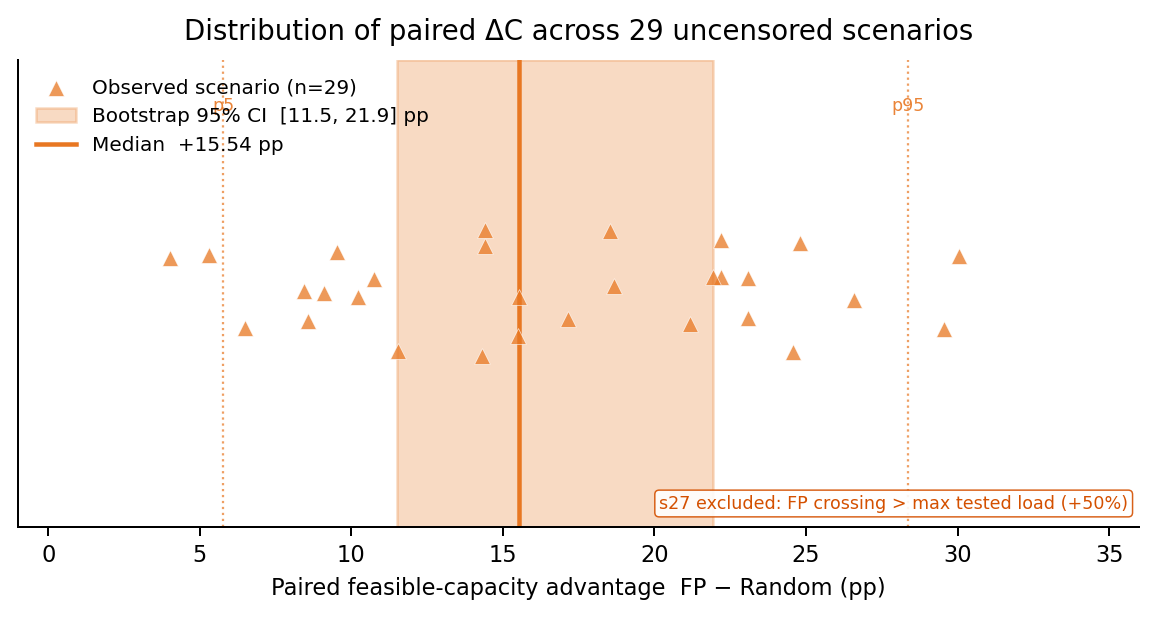
\includegraphics[width=\columnwidth]{fig_mc_dc_dist}
% Source: artifacts/phase1/figures/fig_mc_dc_dist.png (180 dpi; regenerate for camera-ready)
\caption{TODO: Capacity yield crossing illustration. The capacity headroom
percentage ($\lambda$ sweep) for fingerprint-guided and random placement,
showing the conservative bracket separation $\delta_{\mathrm{lo}}$.}
\label{fig:model}
\end{figure}
